%% LyX 2.0.6 created this file.  For more info, see http://www.lyx.org/.
%% Do not edit unless you really know what you are doing.
\documentclass[10pt,twocolumn,british,english,letter]{IEEEtran}
\usepackage[LGR,T1]{fontenc}
\usepackage[latin9]{inputenc}
\usepackage{color}
\definecolor{note_fontcolor}{rgb}{0.80078125, 0.80078125, 0.80078125}
\usepackage{amsthm}
\usepackage{graphicx}

\makeatletter

%%%%%%%%%%%%%%%%%%%%%%%%%%%%%% LyX specific LaTeX commands.
%% The greyedout annotation environment
\newenvironment{lyxgreyedout}
  {\textcolor{note_fontcolor}\bgroup\ignorespaces}
  {\ignorespacesafterend\egroup}

%%%%%%%%%%%%%%%%%%%%%%%%%%%%%% Textclass specific LaTeX commands.
\theoremstyle{plain}
\newtheorem{thm}{\protect\theoremname}
\theoremstyle{definition}
\newtheorem{example}[thm]{\protect\examplename}

%%%%%%%%%%%%%%%%%%%%%%%%%%%%%% User specified LaTeX commands.
\usepackage{babel}

\usepackage{babel}
\addto\captionsbritish{\renewcommand{\examplename}{Example}}
\addto\captionsbritish{\renewcommand{\theoremname}{Theorem}}
\addto\captionsenglish{\renewcommand{\examplename}{Example}}
\addto\captionsenglish{\renewcommand{\theoremname}{Theorem}}
\providecommand{\examplename}{Example}
\providecommand{\theoremname}{Theorem}

\makeatother

\usepackage{babel}
\addto\captionsbritish{\renewcommand{\examplename}{Example}}
\addto\captionsbritish{\renewcommand{\theoremname}{Theorem}}
\addto\captionsenglish{\renewcommand{\examplename}{Example}}
\addto\captionsenglish{\renewcommand{\theoremname}{Theorem}}
\providecommand{\examplename}{Example}
\providecommand{\theoremname}{Theorem}

\begin{document}

\title{{\large{{{Big Data : a tool for research.}}}}}


\date{May 15, 2014}


\author{Ted Brown - Eric Dagobert \\
 Graduate Center (CUNY)}
\maketitle
\begin{abstract}
In this document we are presenting a tool offering features of data
analysis and most importantly predictive modeling in the context of
building data energy management. That is a particular context but
the tool can easily be adapted to any type of data environment.As
of Today, the implementation is made from New-York 's John Jay Building
and contains thousands of data collected from hundreds of sensors
over a period of two years, and regularly updated. 
\end{abstract}

\section*{Introduction}

There are many systems these days that are generating a large amount
of data, some of which needs to be analyzed in real time. Data mining
is now presents in every domain: marketing, finance and medical applications
to name a few. Building management systems are an example of such
a system. They are capable of generating in short time increments,
too much for any operator to examine even retrospectively. In the
mean time this mass of data is correlated, or has cycles, and sometimes
has patterns or trends, upon which analysis should be based.

In this paper we will present a tool that has many features that allow
aspects of the energy use in a building equipped with a modern BAS
system to examine. The tool is based on open source software that
can easily be used by other users for other uses.

\noindent Architecture and design have been motivated by different
constraints and certainly modified several times before reaching the
actual shape. Architecture sits on the following points: speed, easiness
to use and share, and flexibility. We first opted for R Studio that
immediatly offered points 2 and 3 but there was a bottleneck in terms
of performance. We ended up building a website offering python-like
concepts accessible to users.

Here we will first show the contents of this tool and possibilities
of immediate achievement in terms of predictive models. Next section
goes into details relative to implementation and plugin development.
Section 3 presents different case studies in the domain of energy
savings. This is followed by the conclusion.

\includegraphics[clip,scale=0.17]{general}


\section{Background ({*} Note {*} : add references ex. : NREL)}

In general, Building performance energy analysis requires to handle
a large number of data, from multiple sensors placed around every
unit of the heating and cooling system, measuring values at a high
frequency. Therefore, grouping an filtering data is necessary in order
to have different views and extract behaviors of the different variables.
Also, as data analysis must be done on the system dynamics, time is
a very important factor. In the mean time, we know there is some cycles
such as day/night, or week-end/week on which energy performance patterns
are different. It is then very important to extract from data specificities
during those cycles, thus to have dynamic filtering capabilities.

In addition, devices involved in energy propagation are mechanical
and subject to failure. The same goes for sensor, that can without
warning report wrong values. Nevertheless this failures can be detected
and even anticipated with statistical tools such as moving average/moving
standard deviation and autocorrelation. A building performance system
should come with those features.

Energy performance models are not simple. They involve some calculations
often based on derivation and integration. Plus there is so many different
variables that no unique formula exists. Then analysis of complex
functions is often required, for model validation or model verification.
(example : neural network to modelize thermal capacity of a room).

Speaking about models, there too is no unique model that can fit
every building either, not only because building location has an impact on
its energy performance, but also because every building is different
in terms of architecture and material i.e. thermal capacity. Other
factors such as occupancy and seasonality have too a great impact
on the energy model. 

In existing systems, modeling is widely based on curve fitting and
visual analysis of graph. Not only graphs offer at a glance a view
on a large number of data, but most importantely, quickly validate
or invalidate a model.  But given the large amount and nature of data, these graphs
must allow easy changes of time scale as well as the possibility to make comparisons.
Building performance analysis is the task of
high level energy specialists: thus their energy models are based
on differential equations. System therefore has to make possible the
representation of derivatives (difference) and integration (cumulated
sum), and their statistical analysis.

Last but not least, energy performance is a seasonal phenomenon with
hour, day or month cycles. It is then important to extract those cycles
for data analysis, through dynamic filtering.


\section{Our Approach}

Most of existing systems are presenting collected data under the form
of a Dashboard, which will help highlighting key features such as
curve fitting, trending and why not, alerts. We wanted to follow the
same direction by designing a one-page web site that would also allows
sharing of work and information between reseachers.

This dashboard is articulated around three axis : Filtering and defining
a data subset, building the model to analyse, and showing different
statistical points of view. A fourth axis which is learning and predicting
is briefly evocated here and may be the subject of another paper.

\subsection*{Data filters}
Filtering is not only the possibility to eliminate non-representative
(or even biased) values, but it is mainly an easy way to reshape the
time series we want to observe by first of all, accessing the different
facets of a time unit such as hour, day of week, months, year, to
name a few. Then it is possible to restrain the field of observations
to almost any type of time 'buckets'. For example, filtering out summer
data, or week-end data can be easily done.
Furthermore, graphs can contain all the data available and then bring a global view on the system. But  these graphs are displayed within a sliding time window which size and position are managed with a scroll bar, allowing to do zoom in /zoom out on particular periods. This is also convenient for performance as a minimum subset of data is interpolated from and actually displayed.

\subsection*{Statistical tools}

Given the huge amount of data to be processed, we want to offer at
least basic statistical tools such as correlation or moving average
so a user can quickly spot a trend, a relationship between data and
sometimes a dysfunctioning device.(About the last point, showing the
rolling standard deviation of data measured can be very useful to
verify a sensor provides a correct range of values). Simple analysis is immediately available with different graph types : frequency distribution, moving average, moving correlation.
The idea is to provide different levels of analysis for different level of research, from simple analysis to more complex features.\\

Data are modelized as time series, and from there we offer rolling moments and expanding moments. Basically mean, variance, skew and kurtosis are available but also binary moments such as covariance and correlation. Exponentially weighted moments (ewma, ewmvar, etc.)  can also be used. And if this is not sufficient, generic rolling window computation with pre-defined functions can also be done. Among the functions there are boxcar, triangle, Blackman etc. 14 functions are available. Finally users can write their own rolling functions if needed.


\subsection*{Showing Data}

Graphing is the central feature of our system. Classically time series
and frequency distribution are available. We added moving average/standard
dev, correlation, and but also XY which is used to display a value against
another and provides simple curve fitting for model verification, a value could be a serie of data or even an expression of series.
These graphs are of course highly customizable, an operator being able
to display any type of relation. Indeed it is very important to determine relationship between data so we offer easy data manipulation tools to combine series and display together different data sources but also their arithmetic combinations.\\

On top of that, more elaborate mathematic transformations are available
to the user through formulae. That includes the possibility to integrate or derive the values, combine them arithmetically, perform a pattern detection, or any combination of these with the statistical functions described above.

Finally a new concept has been introduced, certainly still under tuning,
that permit to train on and forecast data relationships. Indeed we
added machine learning capabilities in order to compute efficiently
complex thermodynamic events such as building response time (or thermal
capacity) or the impact of the sun on the inside temperature variations.
This has also another objective which is to guess 'hidden variables'
such as the occupancy rate or the outside temperature.


\section{Dynamic Filters}

One objective of this application is to provide different points of
view of the entire dataset . Indeed, with millions of data collected,
filtering then graphing are the best way to represent system states
over time at a glance. Most importantly we want something flexible
enough to accept elaborate requests.

\subsection*{Details of the implementation: the notion of variable.}

The set of data to be analysed is simplifiable down to a  set of variables made of sensors' data projected onto the same time axis.
Prior to display, variables can be re-ordered and filtered. Graphing
several sensors is then graphing the adjusted set.

Before analysis, a subset of sensors is chosen (from a tree) and each
sensor is indexed for convenience (fig.1). The result is seen as
a stack of sensors on which simple operations allowing stack modification
: reorder, delete, add and clear.(fig.2).

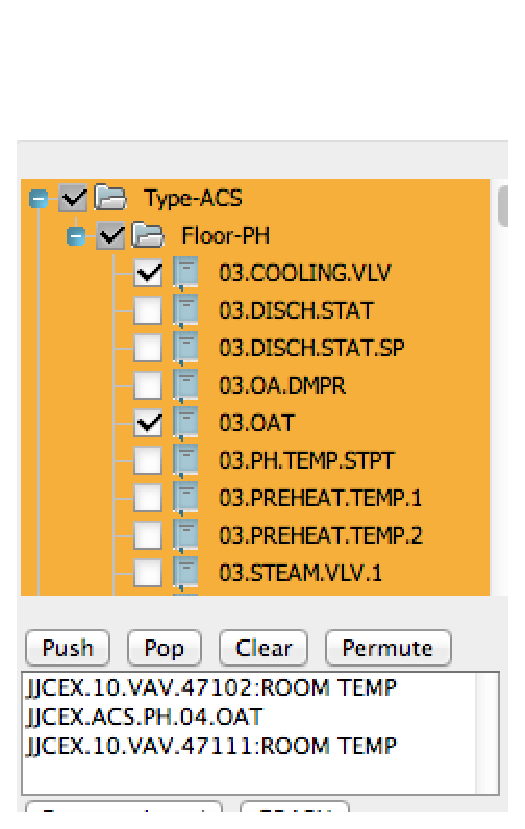
\includegraphics[clip,scale=0.4]{fig1}

Sensor indexing is implicitely made from this stack as the item on
top is number 0, then number 2 . etc.

Indexing has the major advantage of simplifying input as a number
is always easier to input than a long meaningless string. \\
A data serie is therefore represented by a variable, statistically speaking. We will later see the other advantages of such a model.\\

From now on, sensors are designed by their index only. The final data
model is then a set of time series represented by variables \#1, variable \#2,
variable \#3 etc, with a special variable 0 which represents the time axis.\\

\subsection*{Enter into the world of Python}

Behind the scene is Python which has the immense advantage of providing
on-the-fly code compilation and also comes with tons of statistic
and machine learning functions. Rather than building an environment
from scratch and painfully design computation interfaces, we offer
users an entry point inside python code. It is not necessary to know
programing, just be aware of the widely documented open source Python
modules. User will access a safe sandbox where they can design their
own formulas.

Among the Python features available there is Pandas (ref) for the
data model, and Sci-Kit for Machine Learning(ref).


\subsection*{Dynamic Filtering with lambda functions }

What is a lambda function ? Here it is simply a piece of python code
embedded into an unnamed function. In other words, a lambda function
takes a variable  as an input and output its transformation, aligned on the time axis. The code associated to a lambda function
is sent to the server for an on-the-fly evaluation.

We have  two categories of lambda functions : boolean and value.
The first type acts as a filter and the later type is for arithmetic and statistic operations.

As of today, the syntax used to define lambda functions is not obvious,
but this can be later wrapped into simpler code or even widgets, for
a relatively small cost of development.

Filters are boolean lambda functions applied to either the time axis
or each variable. Graphs then display data for which the evaluation
returns True.

This permits a kind of filtering based on all the usual arithmetic
operations plus some Python features and also extra possibilities concerning
time.

Indeed time is modelized with python object and thus offers
all kind of possibilities such as weekend/weekday or leap year. 
\begin{example}
Restrain the data set to the summer months (May, June, July,August)
for which the OAT temperature reaches over 80 degrees: 
\end{example}
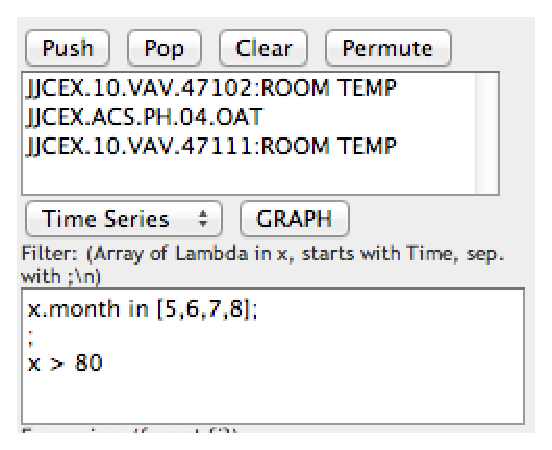
\includegraphics[clip,scale=0.4]{fig2}

Here the first line represents time filtering, and the third line is a condition on the second sensor.

\section{Data transformation and formulae}

Expressions have a slightly different implementation because they
are not reduced to an operation per sensor but they both define the
format and the nature of the output.  Output variables are sub expressions separated with
commas. For instance, if the input is composed of four sensors, the
output can be any combination of one or more variable : \{0\}, \{1\}  will define the output as only the two first series.
In other words, the result displayed is a set of functions of input variables.
All kind of operations on variables are therefore available. We can display
any type of arithmetic (in fact vector operations), e.g. \{0\} + \{1\} will display for every time tick, the sum
of values from sensor 0 and 1. A mean over time can be defined as

\texttt{(\{0\} + \{1\} + \{3\})/3.}

Special index is given to the time axis, called {\texttt{'\{t\}'.}}

The application come with two important useful features for analysis : shift and window. 
First, it is possible to display simultaneously several sensor's data for the same time period, and we added the possibility to individually shift every graph
along the time axis, in order to analysis the correlation, delayed in time, between one or several data sets. For example the Return temperature is a fonction of the supplied
temperature, but the action of one on another may be delayed by the time it takes to propagate updates, so the correlation between these two variables can be computed from one value at t and the other at t+(delay).
The other interesting possibility is to provide rolling statistic moments. Moving average, covariance, skew, and generic window  are available. Users are therefore able to analyse the dynamic components of a system, and analyses the causes of evolution.  

Furthermore transformation on sensor's individual data are made either
with time series builtins or pure Python lambda expressions:

\texttt{\{0\}.apply(lambda x: math.cos(x)) }

will return the cosine of sensor 0 .

Last but not least complex functions of multiple variables can be defined ,
although the syntax is not yet obvious, by using the special variable
'pdata' which represents the entire data set composed of input variables :

\texttt{pdata.apply(lambda x: x{[}1{]} + x{[}2{]} if x{[}0{]}.hour
==2 , axis =1)}

will return sum of sensor 0 and 1 for the period from 2 am to 3 am
every day.

We access to advanced statistic computation such as rolling functions (as explained above) from this point.
For instance :

\texttt{pandas.rolling\_cov(\{0\},\{1\},window=4)}

will display covariance of sensors 0 and 1 computed over a rolling
period of four ticks.



\section*{Analysis at a glance: types of graph }
The application handle three different sources of data to be displayed : raw, transformed and predicted. The raw data correspond to those coming directly from the sensors, without transformation, but can eventually be filtered. Then the operator can choose to do computations with data and results are displayed along the sources. Finally, an expression of data can be used for training and results of training as well as forecast are shown together.
Different types of graphs are available to higlight different type of information:

\begin{itemize}
\item Combined time serie : graph of one or several expressions using time as x-axis. (Sometime a rescaling is necessary).
\item XY: merges two dataseries along time axis and displays one as function of the other.
\item Correlation: This is a quick access to correlation computations, the graphs displayed here are the rolling correlations of every sensors compared to the first one.
\item Histogram: Displays the distribution relative to the first variable. 
\item Timeserie + moving average and standard deviation: displays what is also called "Bollinger bands" i.e. moving average accompanied by two standard deviations. This can be used to detect an abnormal behavior of a sensor.
\item Table : Displays a table that can be downloaded as a csv file.

\end{itemize}
\begin{lyxgreyedout}
\section*{Advanced features : Python plugins}
For advanced users, it is possible to upload python code that will be compiled on-the-fly and immediately accessible via the Expression box. This is convenient for fast prototyping and tuning, and eventually can be an entry point for python client applications. 

\section*{Training and prediction for research}

advantages: 
\begin{itemize}
\item quickly determine whether there is a relation between different measured
values (on a given timeslice) 
\item can try different machine types, different training sets and different
training size 
\item results can be reinjected into another expression -> model verif 
\item sharing of results 
\end{itemize}
sits on python scikit outputs consistent with data model -> used for
feedback


\section*{ Case studies go here}

-simple case : room temp with OAT and time of day -energy propagation
from emitter to sensors : SVM (add figures)


\section*{Conclusion}

Users : researchers goals: energy savings, dysfunctionment prevention%
\end{lyxgreyedout}

\end{document}
